% 原始两面板及数据保持不变；翻译标题、轴题和图例标题。
\begin{tikzpicture}
\node[anchor=south west,inner sep=0] (plot) at (0,0) {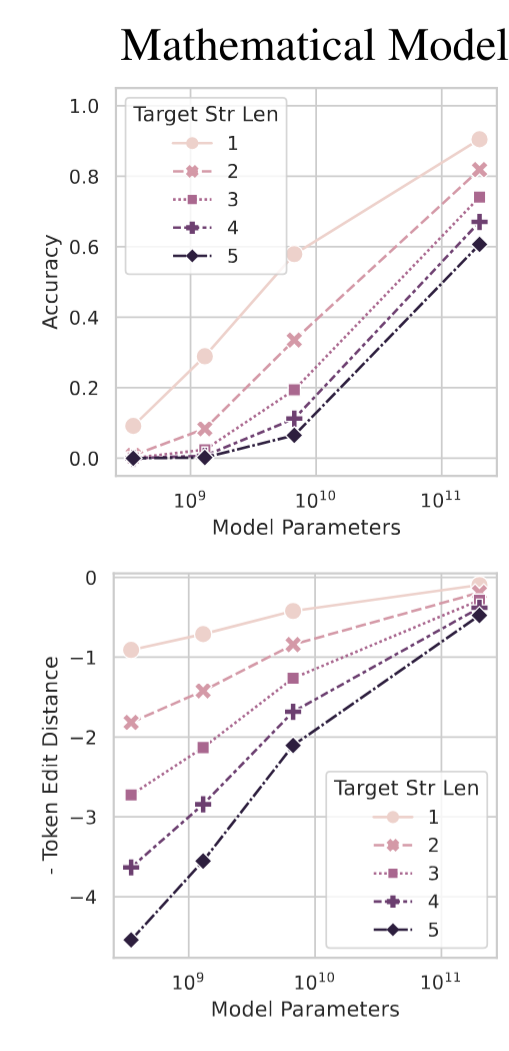
\includegraphics[width=.36\linewidth]{part1/visuals/token_edit.png}};
\begin{scope}[x={(plot.south east)},y={(plot.north west)},every node/.style={font=\scriptsize,inner sep=0pt}]
\fill[white] (.18,.932) rectangle (1,1);
\node[font=\small] at (.59,.966) {数学模型};
\fill[white] (.04,.61) rectangle (.13,.80);
\node[rotate=90] at (.09,.705) {准确率};
\fill[white] (.31,.480) rectangle (.92,.515);
\node at (.615,.497) {模型参数量};
\fill[white] (.25,.879) rectangle (.56,.91);
\node at (.405,.894) {目标字符串长度};
\fill[white] (.04,.15) rectangle (.13,.38);
\node[rotate=90] at (.09,.265) {负词元编辑距离};
\fill[white] (.31,.018) rectangle (.92,.055);
\node at (.615,.037) {模型参数量};
\fill[white] (.65,.235) rectangle (.97,.266);
\node at (.81,.251) {目标字符串长度};
\end{scope}
\end{tikzpicture}
